\documentclass{beamer}

\mode<presentation>
{
  \usetheme{CambridgeUS}
  \setbeamercovered{invisible}
}

\usepackage[english]{babel}
\usepackage[latin1]{inputenc}
\usepackage{times}
\usepackage[T1]{fontenc} 
% Or whatever. Note that the encoding and the font should match. If T1
% does not look nice, try deleting the line with the fontenc.
\usepackage{amsmath}

\newcommand{\linespace}{\vskip 0.25cm}

% The text in square brackets is the short version of your title and will be used in the
% header/footer depending on your theme.
\title{A detailed analysis of a PushGP run}
%{Using Graph Databases to Explore Genetic Programming Run Dynamics}

% Sub-titles are optional - uncomment and edit the next line if you want one.
\subtitle{Rooting through the relics of digital evolution} 

% The text in square brackets is the short version of your name(s) and will be used in the
% header/footer depending on your theme.
\author[Nic McPhee]{Nic McPhee (w/ Finzel, Casale, Helmuth, \& Spector)}

% The text in square brackets is the short version of your institution and will be used in the
% header/footer depending on your theme.
\institute[UMN Morris]
{
  Division of Science and Mathematics \\
  University of Minnesota, Morris \\
  Morris, Minnesota, USA \\
}

% The text in square brackets is the short version of the date if you need that.
\date[May 2016, GPTP, Ann Arbor MI] % (optional)
{May 2016 \\ Genetic Programming Theory and Practice \\ University of Michigan \\ Ann Arbor, MI}

% Delete this, if you do not want the table of contents to pop up at
% the beginning of each subsection:
\AtBeginSection[]
{
  \begin{frame}<beamer>
    \frametitle{Outline}
    \tableofcontents[currentsection, hideothersubsections]
  \end{frame}
}

\begin{document}

\begin{frame}
  \titlepage
\end{frame}

% For a 20-25 minute senior seminar talk you probably want something like:
% - Two or three major sections (other than the summary).
% - At *most* three subsections per section.
% - Talk about 30s to 2min per frame. So there should probably be between
%   15 and 30 frames, all told.

\section*{Overview}

\subsection*{The Big Picture}

\begin{frame}
  \frametitle{The Big Picture}
  
  \begin{itemize}
	\item Genetic programming clearly \emph{works}.
	\item But we rarely know \emph{why} or \emph{how}.
	\item Databases allow examination of the internal interactions of a run.
	\item Graph databases allow us to collect and analyze lineages.
	\item Silico-paleontology can help us understand and improve our tools.
  \end{itemize}

\end{frame}

\subsection*{Outline}

\begin{frame}
  \frametitle{Outline}
  \tableofcontents[hideallsubsections]
\end{frame}

\section{What do we know? (And how do we talk about it?)}

\subsection{We throw so much away}

\begin{frame}{We keep/see/share so little}
			EC research has the potential to generate \emph{huge} amounts of data.
			\linespace
			What do we normally do with that data?
			\linespace
			We typically throw it away -- \& paleontologists weep!
			\linespace
			\centering
			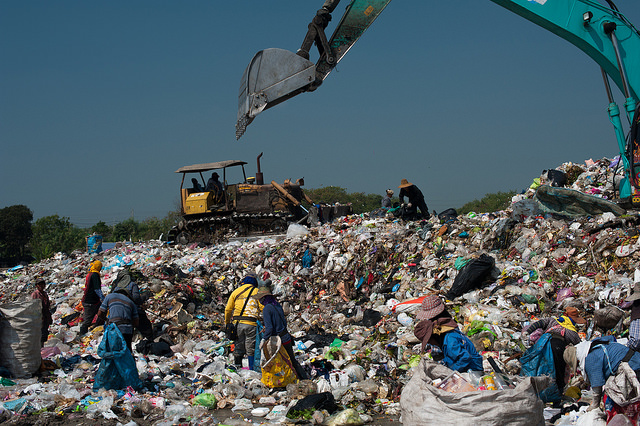
\includegraphics[width = 0.6 \linewidth]{../../figures/Harvest.jpg} \\
			\tiny{\url{https://www.flickr.com/photos/thibaud_saintin/12533059215/}}
			% \textbf{Get bulldozer on dump photo}
\end{frame}

\subsection{Let's go hunting for beetles!}

\begin{frame}{Let's trade the forest for the trees}
	We typically share summary results (tables, graphs) that represent a 30,000 foot view of (part of) the forest.
	\linespace
	We'll instead focus on a single tree, in places peeling back the bark and poking at the beetles we find underneath.
	\linespace
	\linespace
	This is not a ``one or the other'' question. There is important value in understanding
	the behavior of large-scale ecosystems, as well as understanding the details of
	organisms in those ecosystems.
\end{frame}

\section{Tools, problem, and setup}

\begin{frame}{PushGP/Clojush}
	\begin{itemize}
		\item PushGP: Stack-based GP system; multiple types; successful in a variety of domains
		\item Plush genomes: More in Lee's talk; linear representation that maps to structured Push programs.
		\item Operators: Alternation (form of n-point crossover with shifts), ``point'' mutation, and \emph{close} mutation
		\item Lexicase selection: Avoid aggregation; shuffle test cases afresh for each selection and select lexicographically using that ordering
		\item Population size = 1,000
	\end{itemize}
	The example here uses PushGP, etc., but could be applied to most any evolutionary system.
\end{frame}

\begin{frame}{Replace-space-with-newline problem}
	Replace-space-with-newline is from software synthesis benchmark suite that was central to Tom Helmuth's dissertation last year.
	\begin{itemize}
		\item Two related goals. Given an input string:
		\begin{itemize}
			\item \emph{Print} the string with all the spaces replaced by newlines.
			\item \emph{Return} (on the \texttt{integer} stack) the number of \emph{non-space} characters in the input string.
		\end{itemize}
		\item Error vector with 200 values, one for each type of error across 100 test cases
	\end{itemize}
	
	This problem has a roughly 50\% success rate with described setup.
	\linespace
	We'll focus on a run that succeeded quickly (20 generations)
\end{frame}

\begin{frame}{DB \& visualization tools}
	Graph database tools:
	\begin{itemize}
		\item Titan graph database (an Apache project)
		\item Tinkerpop graph query language
		\item Gremlin shell
	\end{itemize}
	\linespace
	Graph visualizations created with Graphviz.
\end{frame}

\section{Visualizing ancestries}

\subsection{Full ancestry graphs}

\begin{frame}{Full ancestry of ``winners''}
	\centering
	\includegraphics[width=\linewidth]{../../figures/run0_GPTP_2_font_40}
\end{frame}

\begin{frame}{Full ancestry of ``winners'' (sized and colored)}
		\begin{overprint}
		\onslide<1-3> 			\centering
		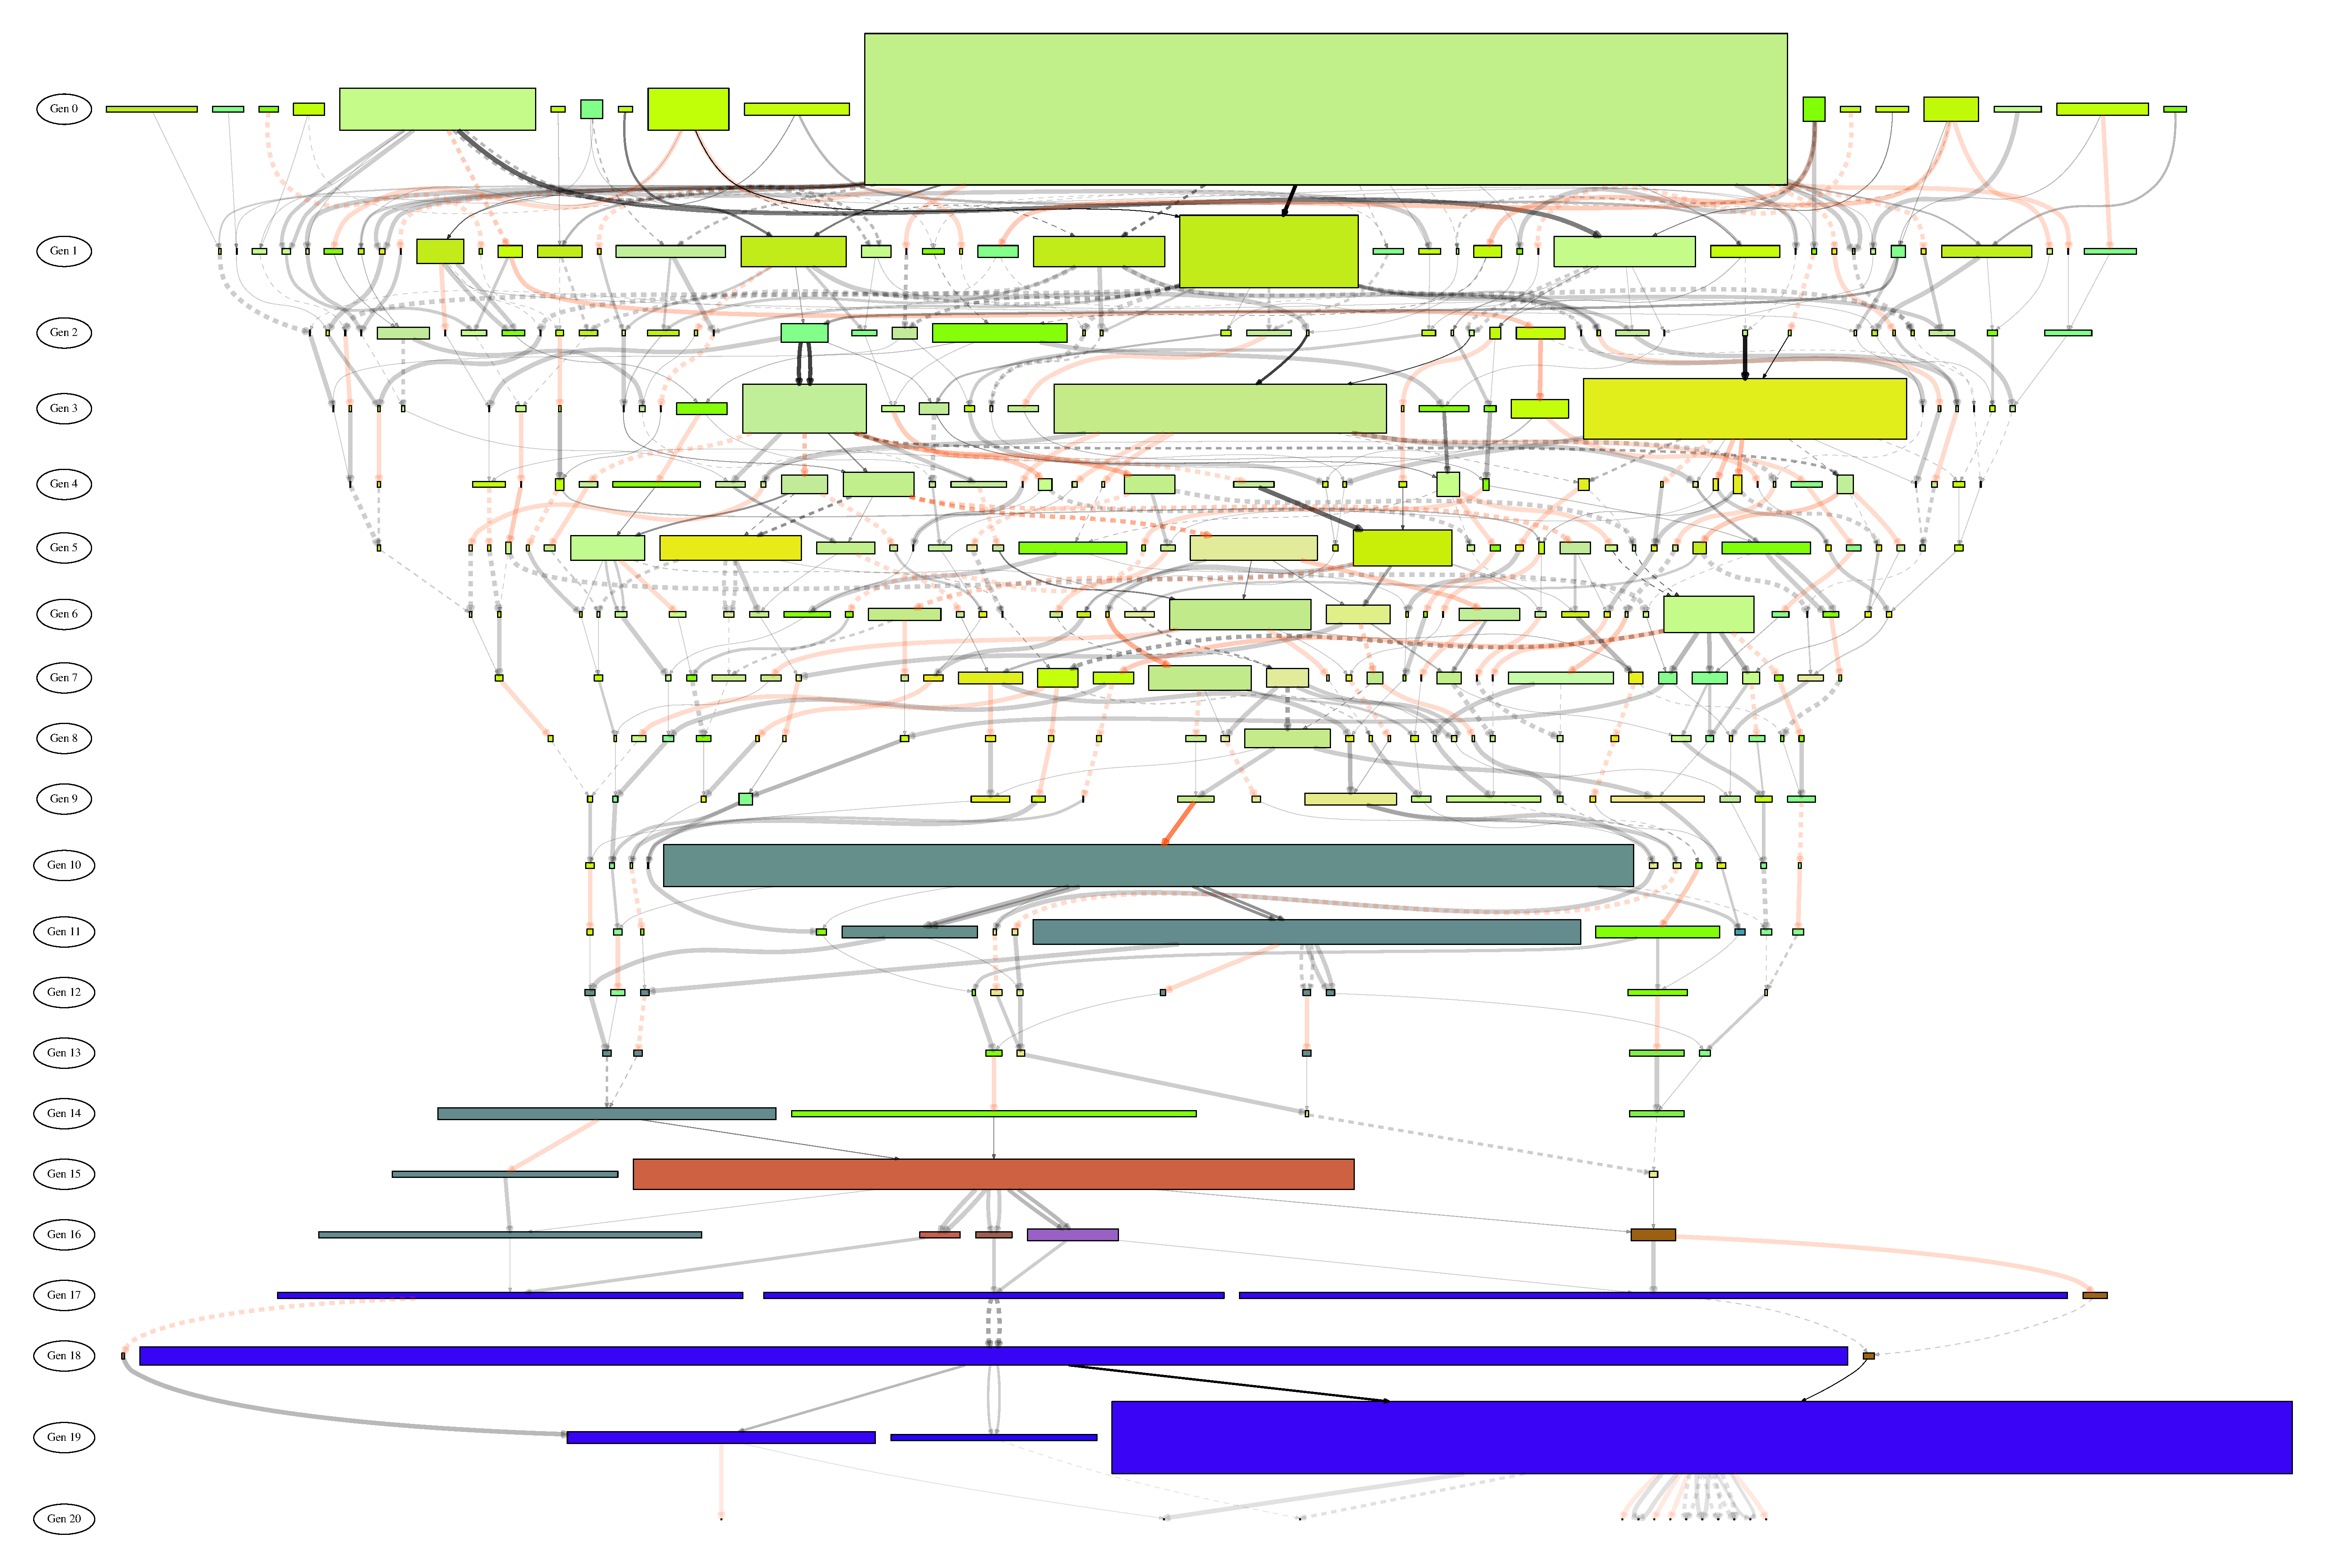
\includegraphics[width=0.7\linewidth]{../../figures/run0_RBM_color_full_30000}
		\onslide<4> 			\centering
		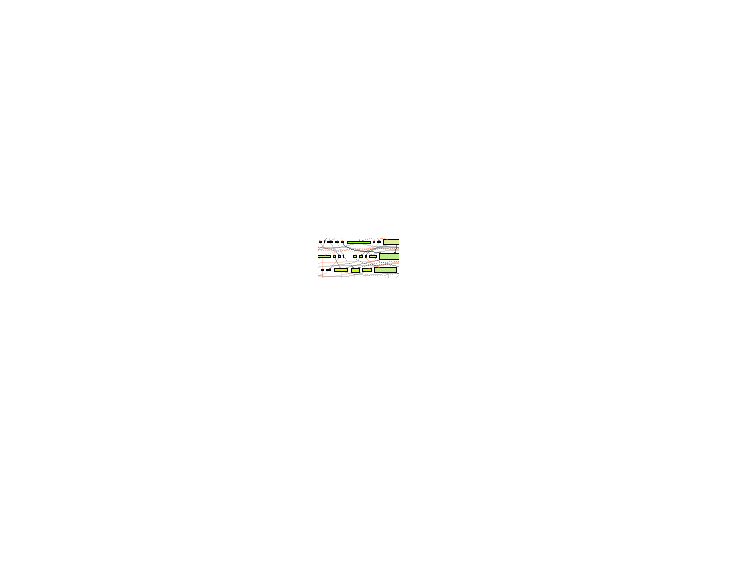
\includegraphics[width=0.9\linewidth]{../../figures/run0_colored_detail}
		\end{overprint}
	\begin{overprint}
		\onslide<1>
		Width of boxes is proportional to number of selections
		\onslide<2>
		Heights are proportional to number of children \emph{in this graph}
		\onslide<3>
		Colors are a compression of the \emph{error vectors} (200 errors to RGB colors)
		\onslide<4>
		Edges encode genetic ops and level of genetic contribution of parents
	\end{overprint}
\end{frame}

\subsection{Filtering ancestries}

\begin{frame}{Why we want to filter ancestries}
	\begin{center}
	\includegraphics[width=\linewidth]{../../figures/run0_GPTP_2_font_40}
	\end{center}
	\linespace
	Busy and dense, even for a very short run like this
\end{frame}

\begin{frame}{Why we want to filter ancestries}
	\begin{columns}
		\begin{column}{0.4 \linewidth}
			Vastly worse for longer runs like this! (129 generations)
			\linespace
			And we have much bigger data sets than this, with thousands of generations
			\linespace
			So let's try to filter the ancestries to focus on the individuals ``that matter''.
		\end{column}
		\begin{column}{0.6 \linewidth}
\begin{center}
	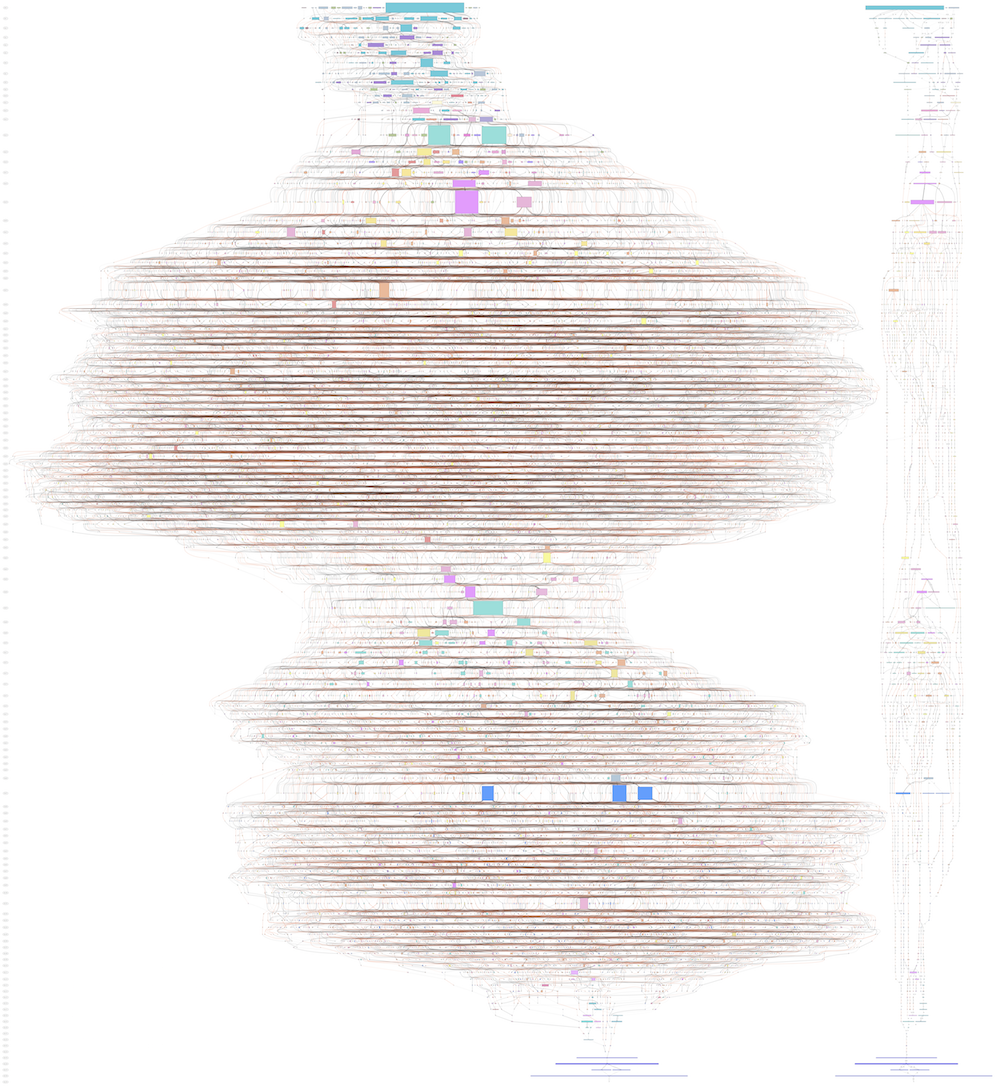
\includegraphics[height=0.8\textheight]{../../figures/run1_RBM_color_filtered_and_full_60000.png}
\end{center}
\end{column}			
	\end{columns}
\end{frame}

\begin{frame}{A simplistic approach to filtering}
	We want to focus on the individuals that contributed the most to their offspring.
	\linespace
	Compute the Damerau-Levenshtein distance between parent-child genomes and eliminate ``far'' parent if:
	\begin{itemize}
		\item The ``near'' parent is \emph{very} near (so it contributes all or almost all the genetic material)
		\item The ``far'' parent is at least twice as far as the ``near'' parent
	\end{itemize}
	These are really a simplistic hack to let us quickly focus on what are \emph{likely} to be the most important parts of the graph, but they can oversimplify (as we'll see later).
\end{frame}

\begin{frame}{Filtered version of our target run}
	\begin{center}
		
\includegraphics[width=\linewidth]{../../figures/run0_RBM_color_filtered_and_full_30000}
	\end{center}
\end{frame}

\section{Exploring a run in detail}

\subsection{A successful program}

\begin{frame}{A successful program}
	There are 13 successful individuals in the final generation.
	\linespace
	Pick 20:435 to focus on:
	\begin{itemize}
		\item Constructed via mutation of 3 instructions from 19:554
		\item Genome has 194 instructions
		\item Simplified program has 9 instructions \& is quite readable
	\end{itemize}
	\linespace
	\texttt{(\textbackslash space  \textbackslash newline in1 string\_replacechar print\_string}\\
	\texttt{\quad in1 \textbackslash space string\_removechar string\_length)}
	\linespace
	\begin{overprint}
		\onslide<1>
		We'll focus on these 9 instructions \emph{recognizing that there are huge assumptions here}.
		\onslide<2>
		First 5 instructions do the ``printing''
		\onslide<3>
		Last 4 instructions do the ``returning''
	\end{overprint}
\end{frame}

\subsection{Ancestry graph successful, simplified program}

\begin{frame}{Exploring a run in detail}
	
	\begin{columns}
		\begin{column}{0.4 \linewidth}
			\centering
			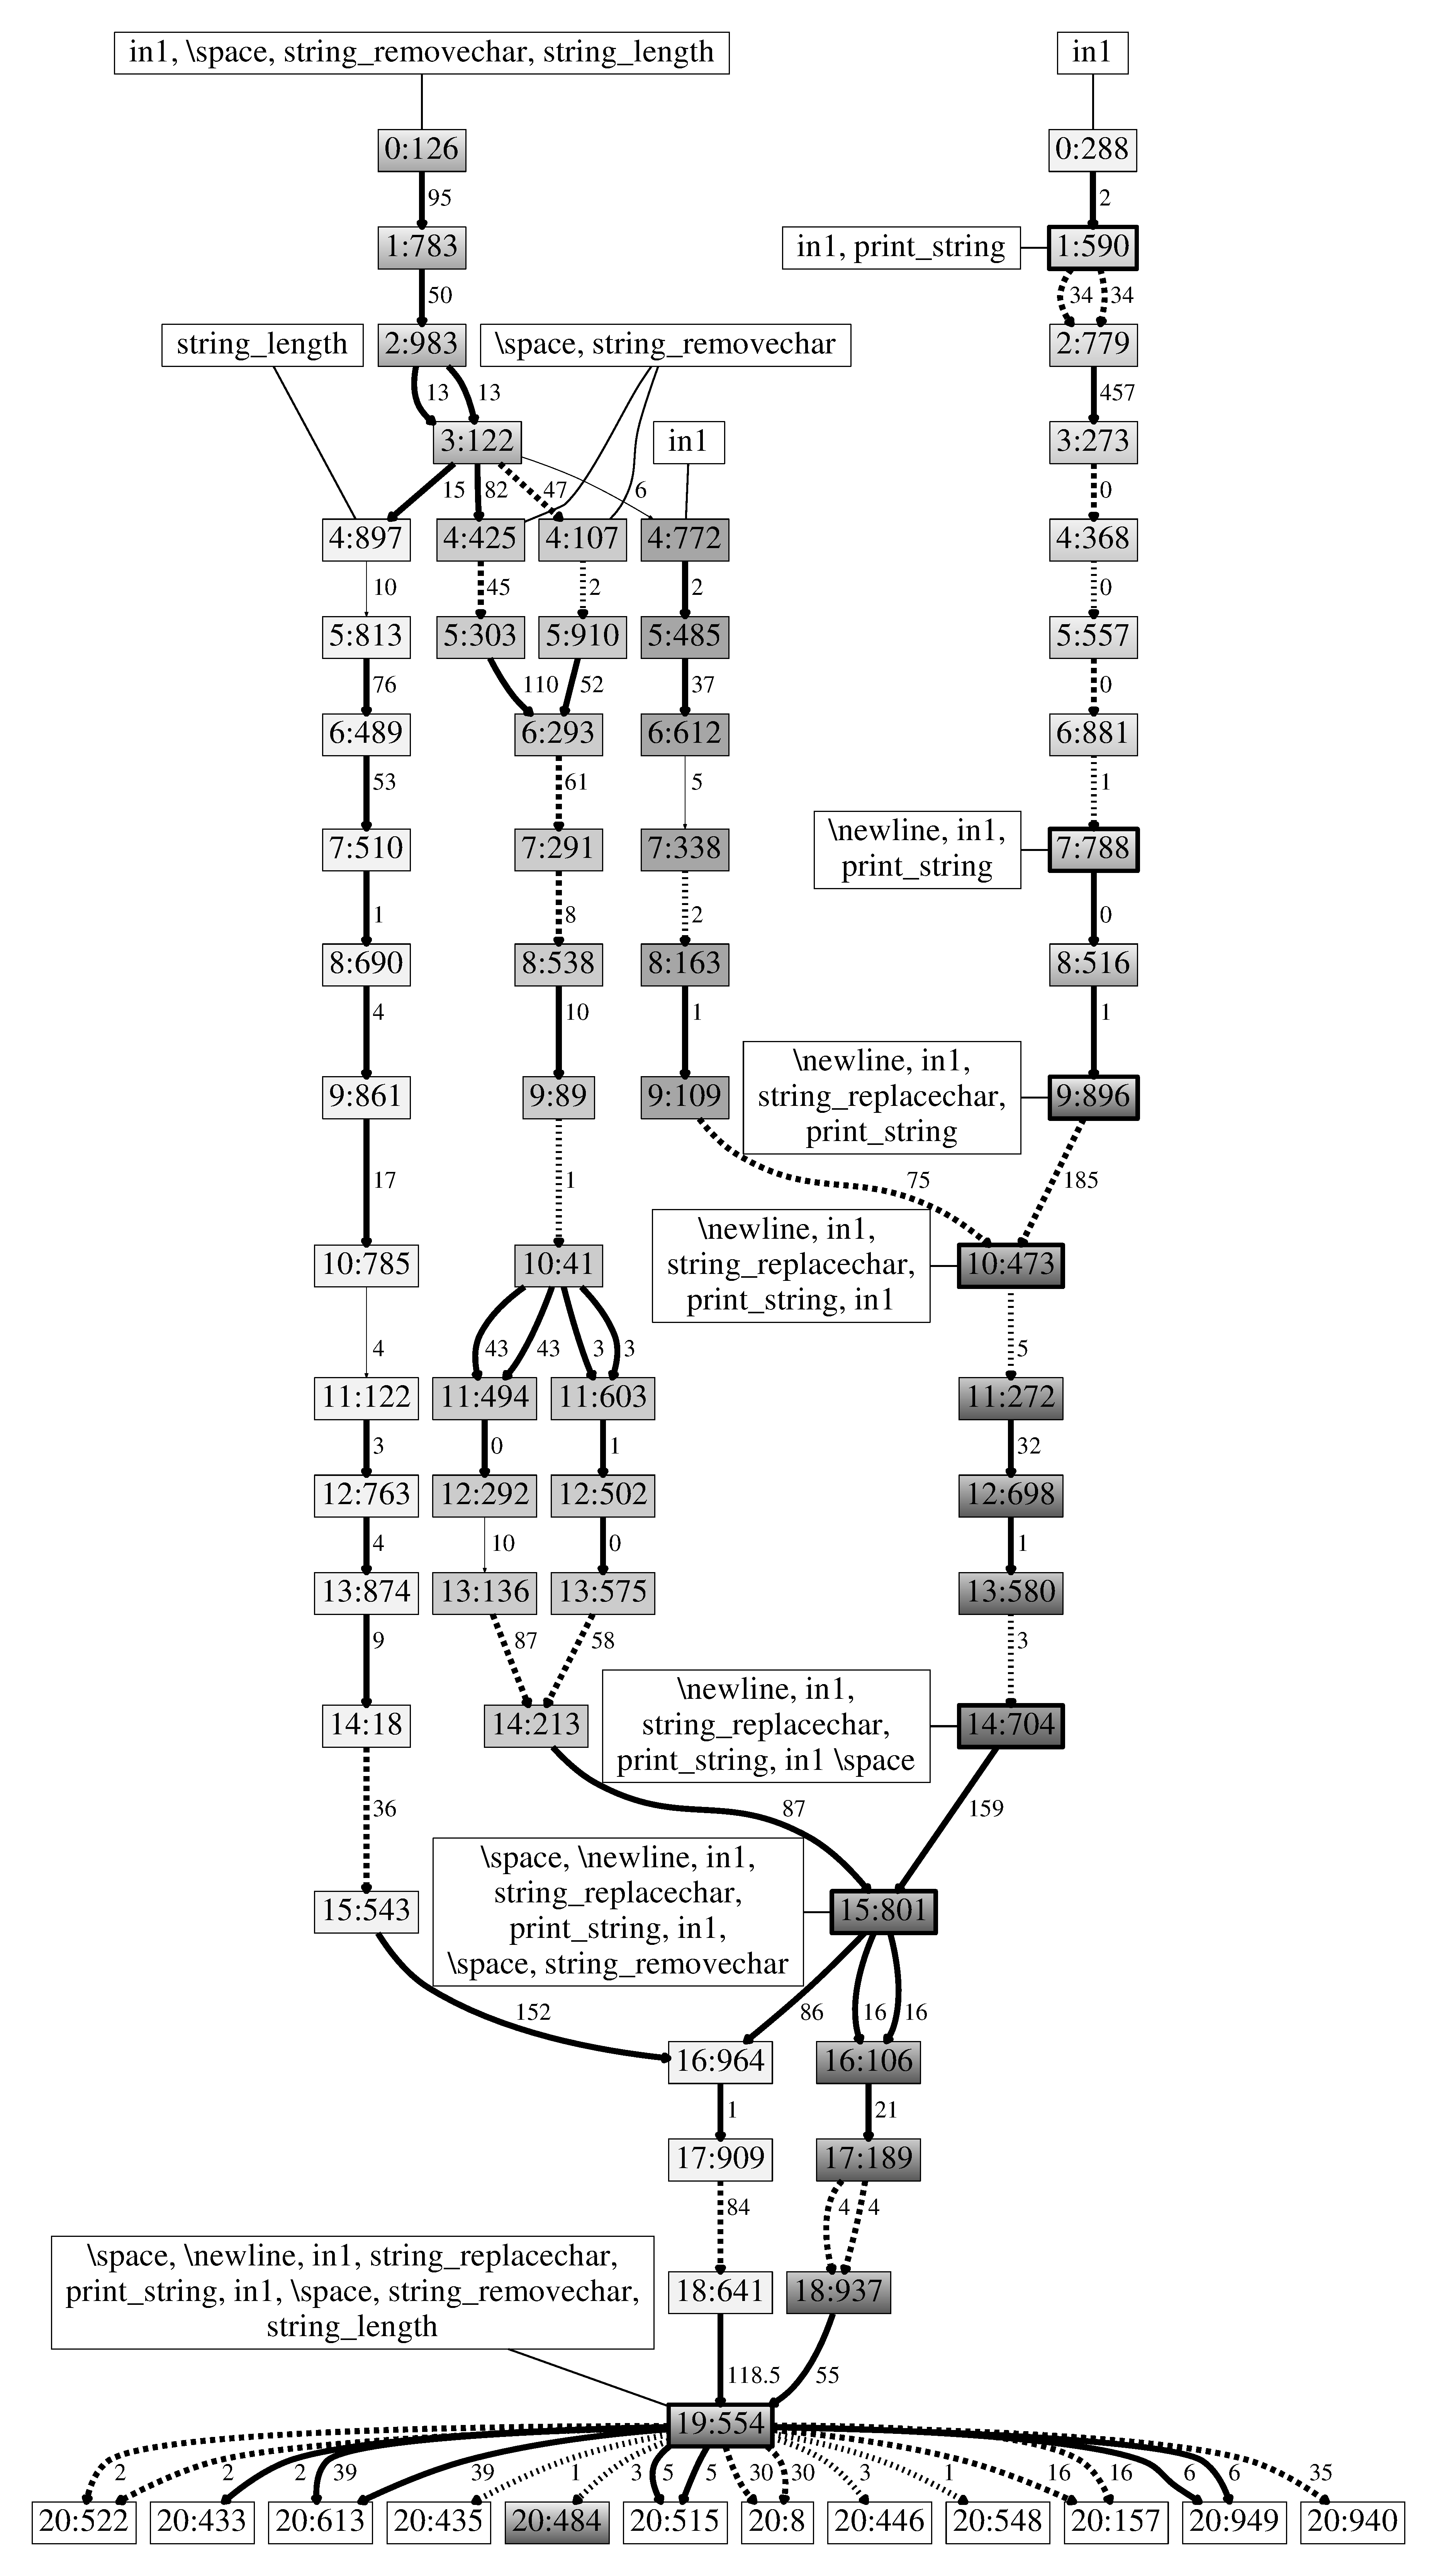
\includegraphics[height = 0.8 \textheight]{../../figures/filtered_fill.pdf}
		\end{column}
		
		\begin{column}{0.6 \linewidth}
			\begin{overprint}
				\onslide<1>
				\textbf{Ignore graph on this slide -- I'll hand out printed copies}
				\linespace
				\textbf{Go over how to ``read'' the graph}
				\onslide<2>
				We traced back the origin of every one of these 9 instructions
				\linespace
				This isn't whole story, but it's a story we can tell
				\linespace
				(Counter) example: Removing extraneous \texttt{print\_newline} ``fixes'' 100 test cases.
			\end{overprint}
		\end{column}
	\end{columns}
\end{frame}

\begin{frame}{First 5 instructions: Printing}
	
	\begin{columns}
		\begin{column}{0.4 \linewidth}
			\centering
			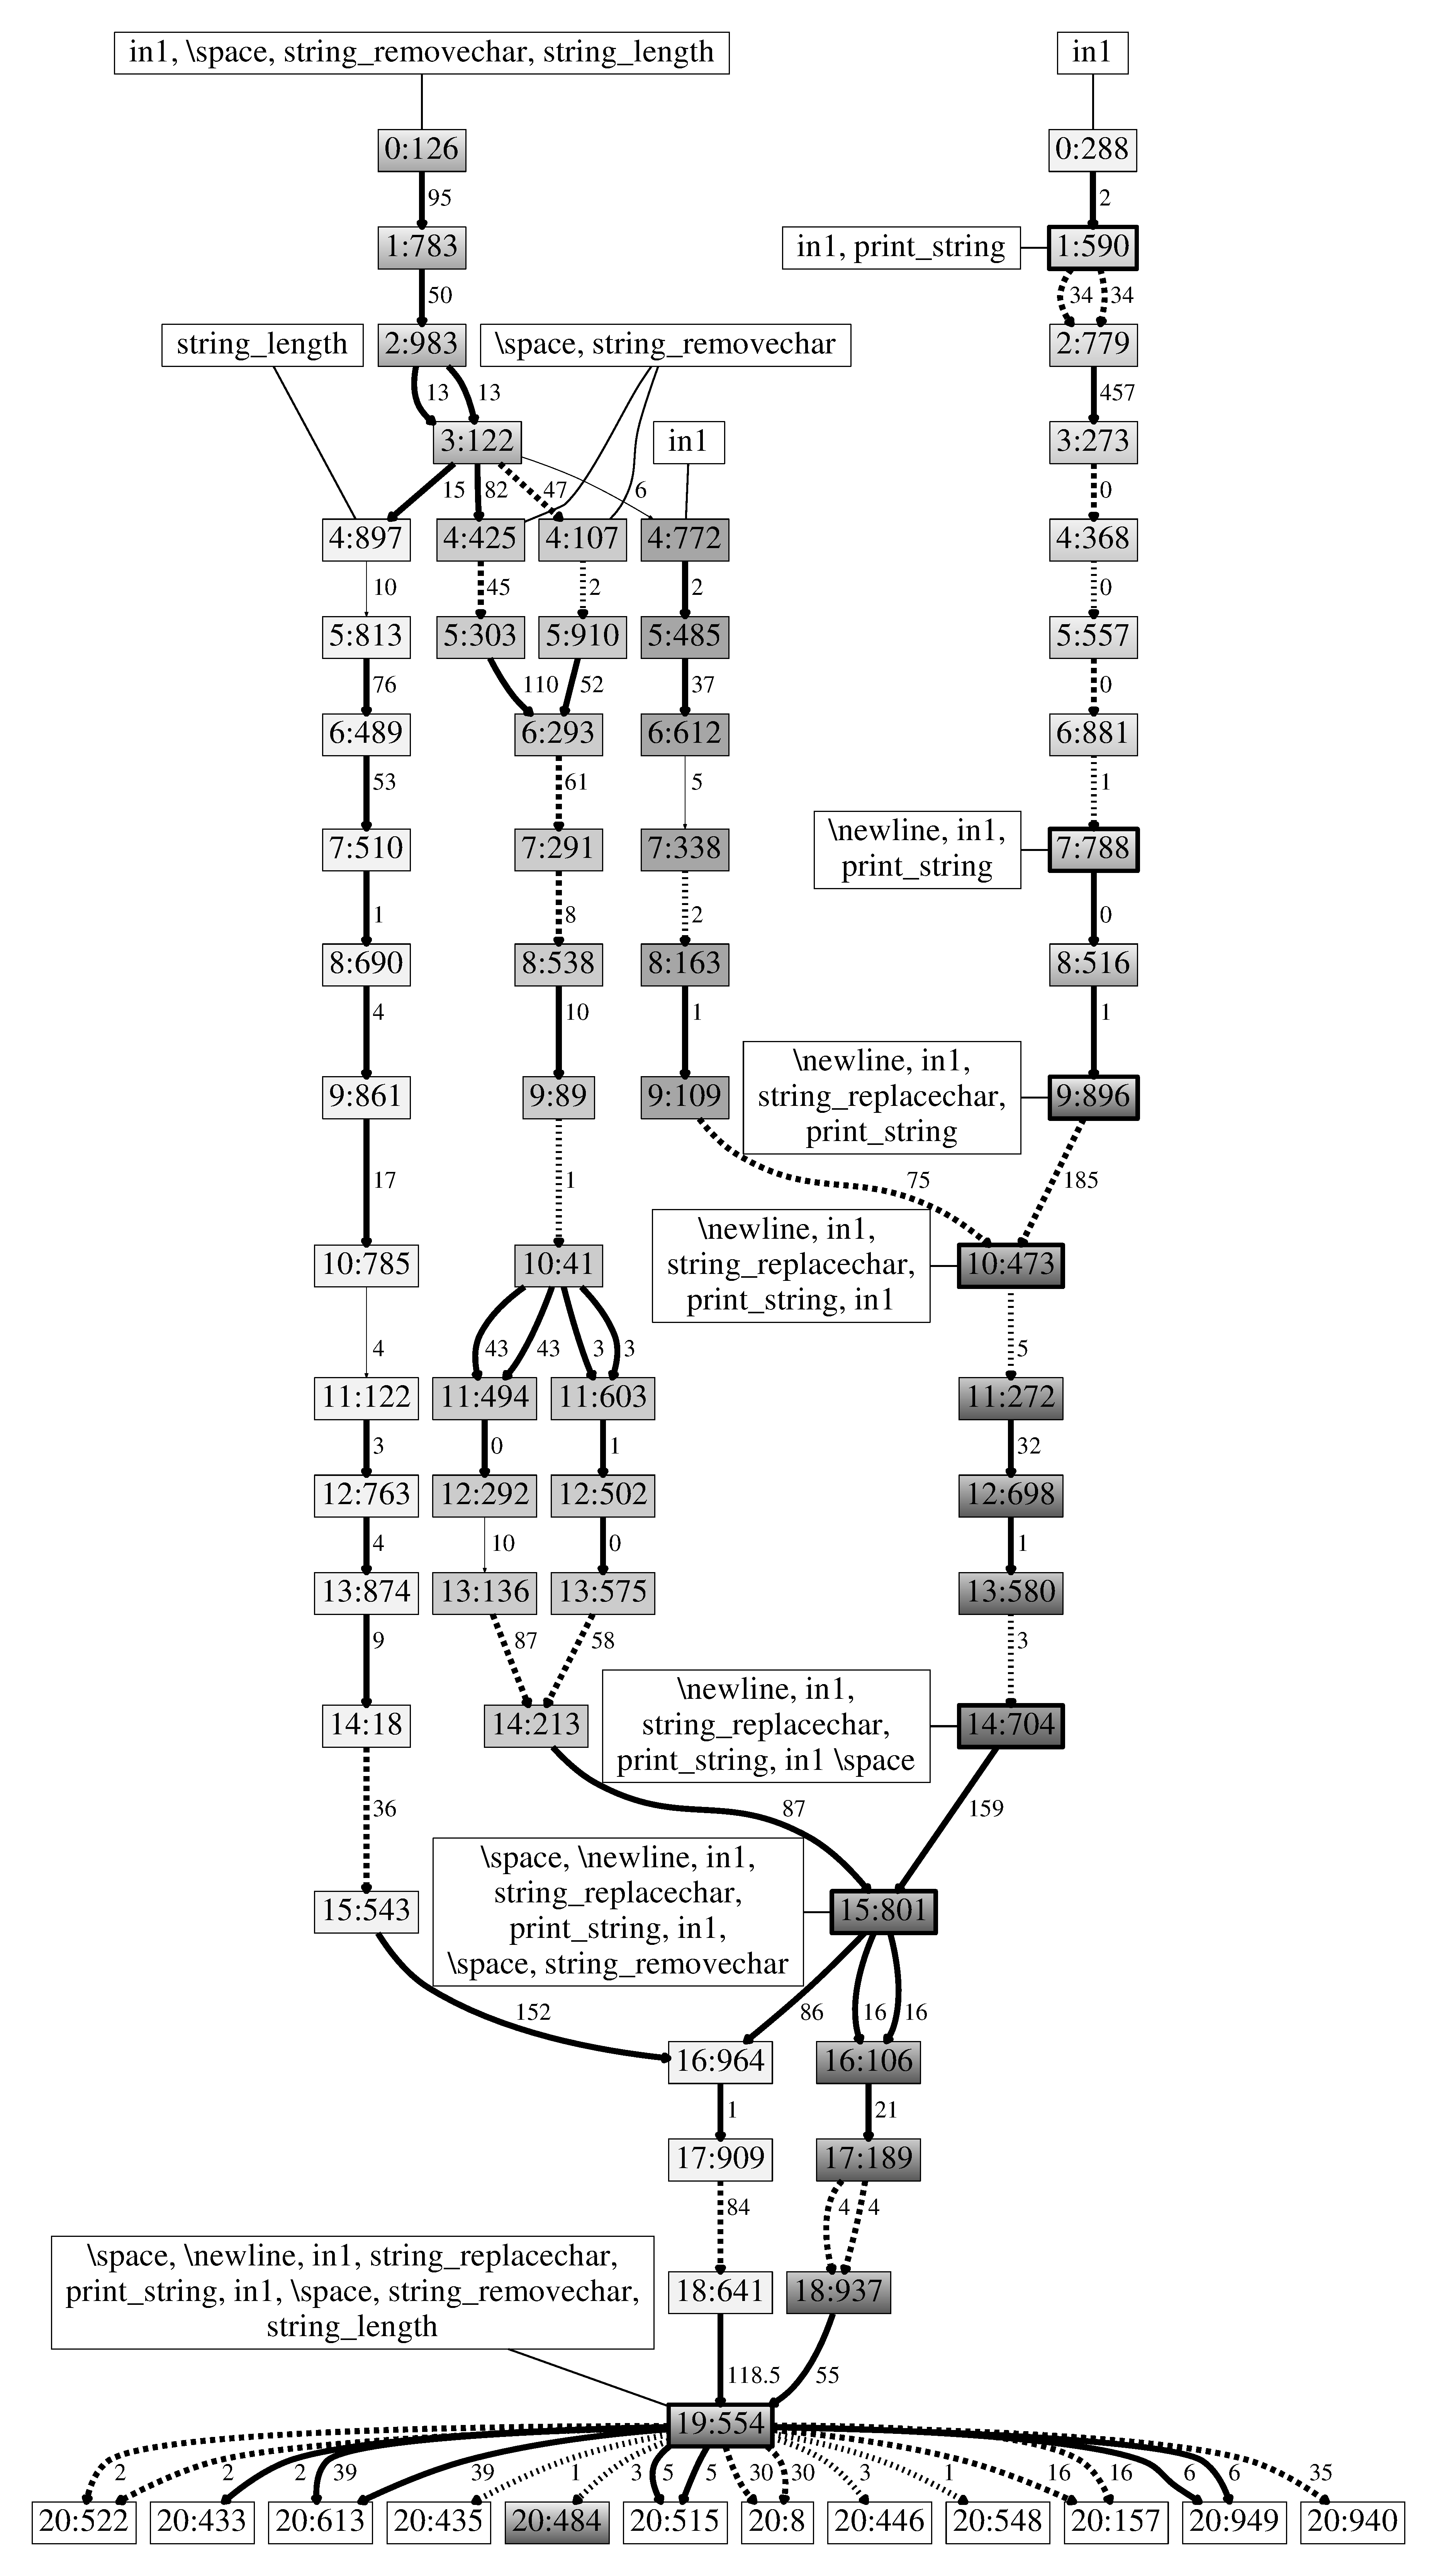
\includegraphics[height = 0.8 \textheight]{../../figures/filtered_fill.pdf}
		\end{column}
		
		\begin{column}{0.6 \linewidth}
			Only one of the 5 ``printing'' instructions was present in the initial generation (an \texttt{in1})
			\linespace
			\emph{Each of the other 4 were introduced via mutation!}
			\linespace
			Introductions range from generation 1 (a \texttt{print\_string}) to generation 14
			\linespace
			Right hand branch in the graph
		\end{column}
	\end{columns}
\end{frame}

\begin{frame}{Last 4 instructions: Returning}
	
	\begin{columns}
		\begin{column}{0.4 \linewidth}
			\centering
			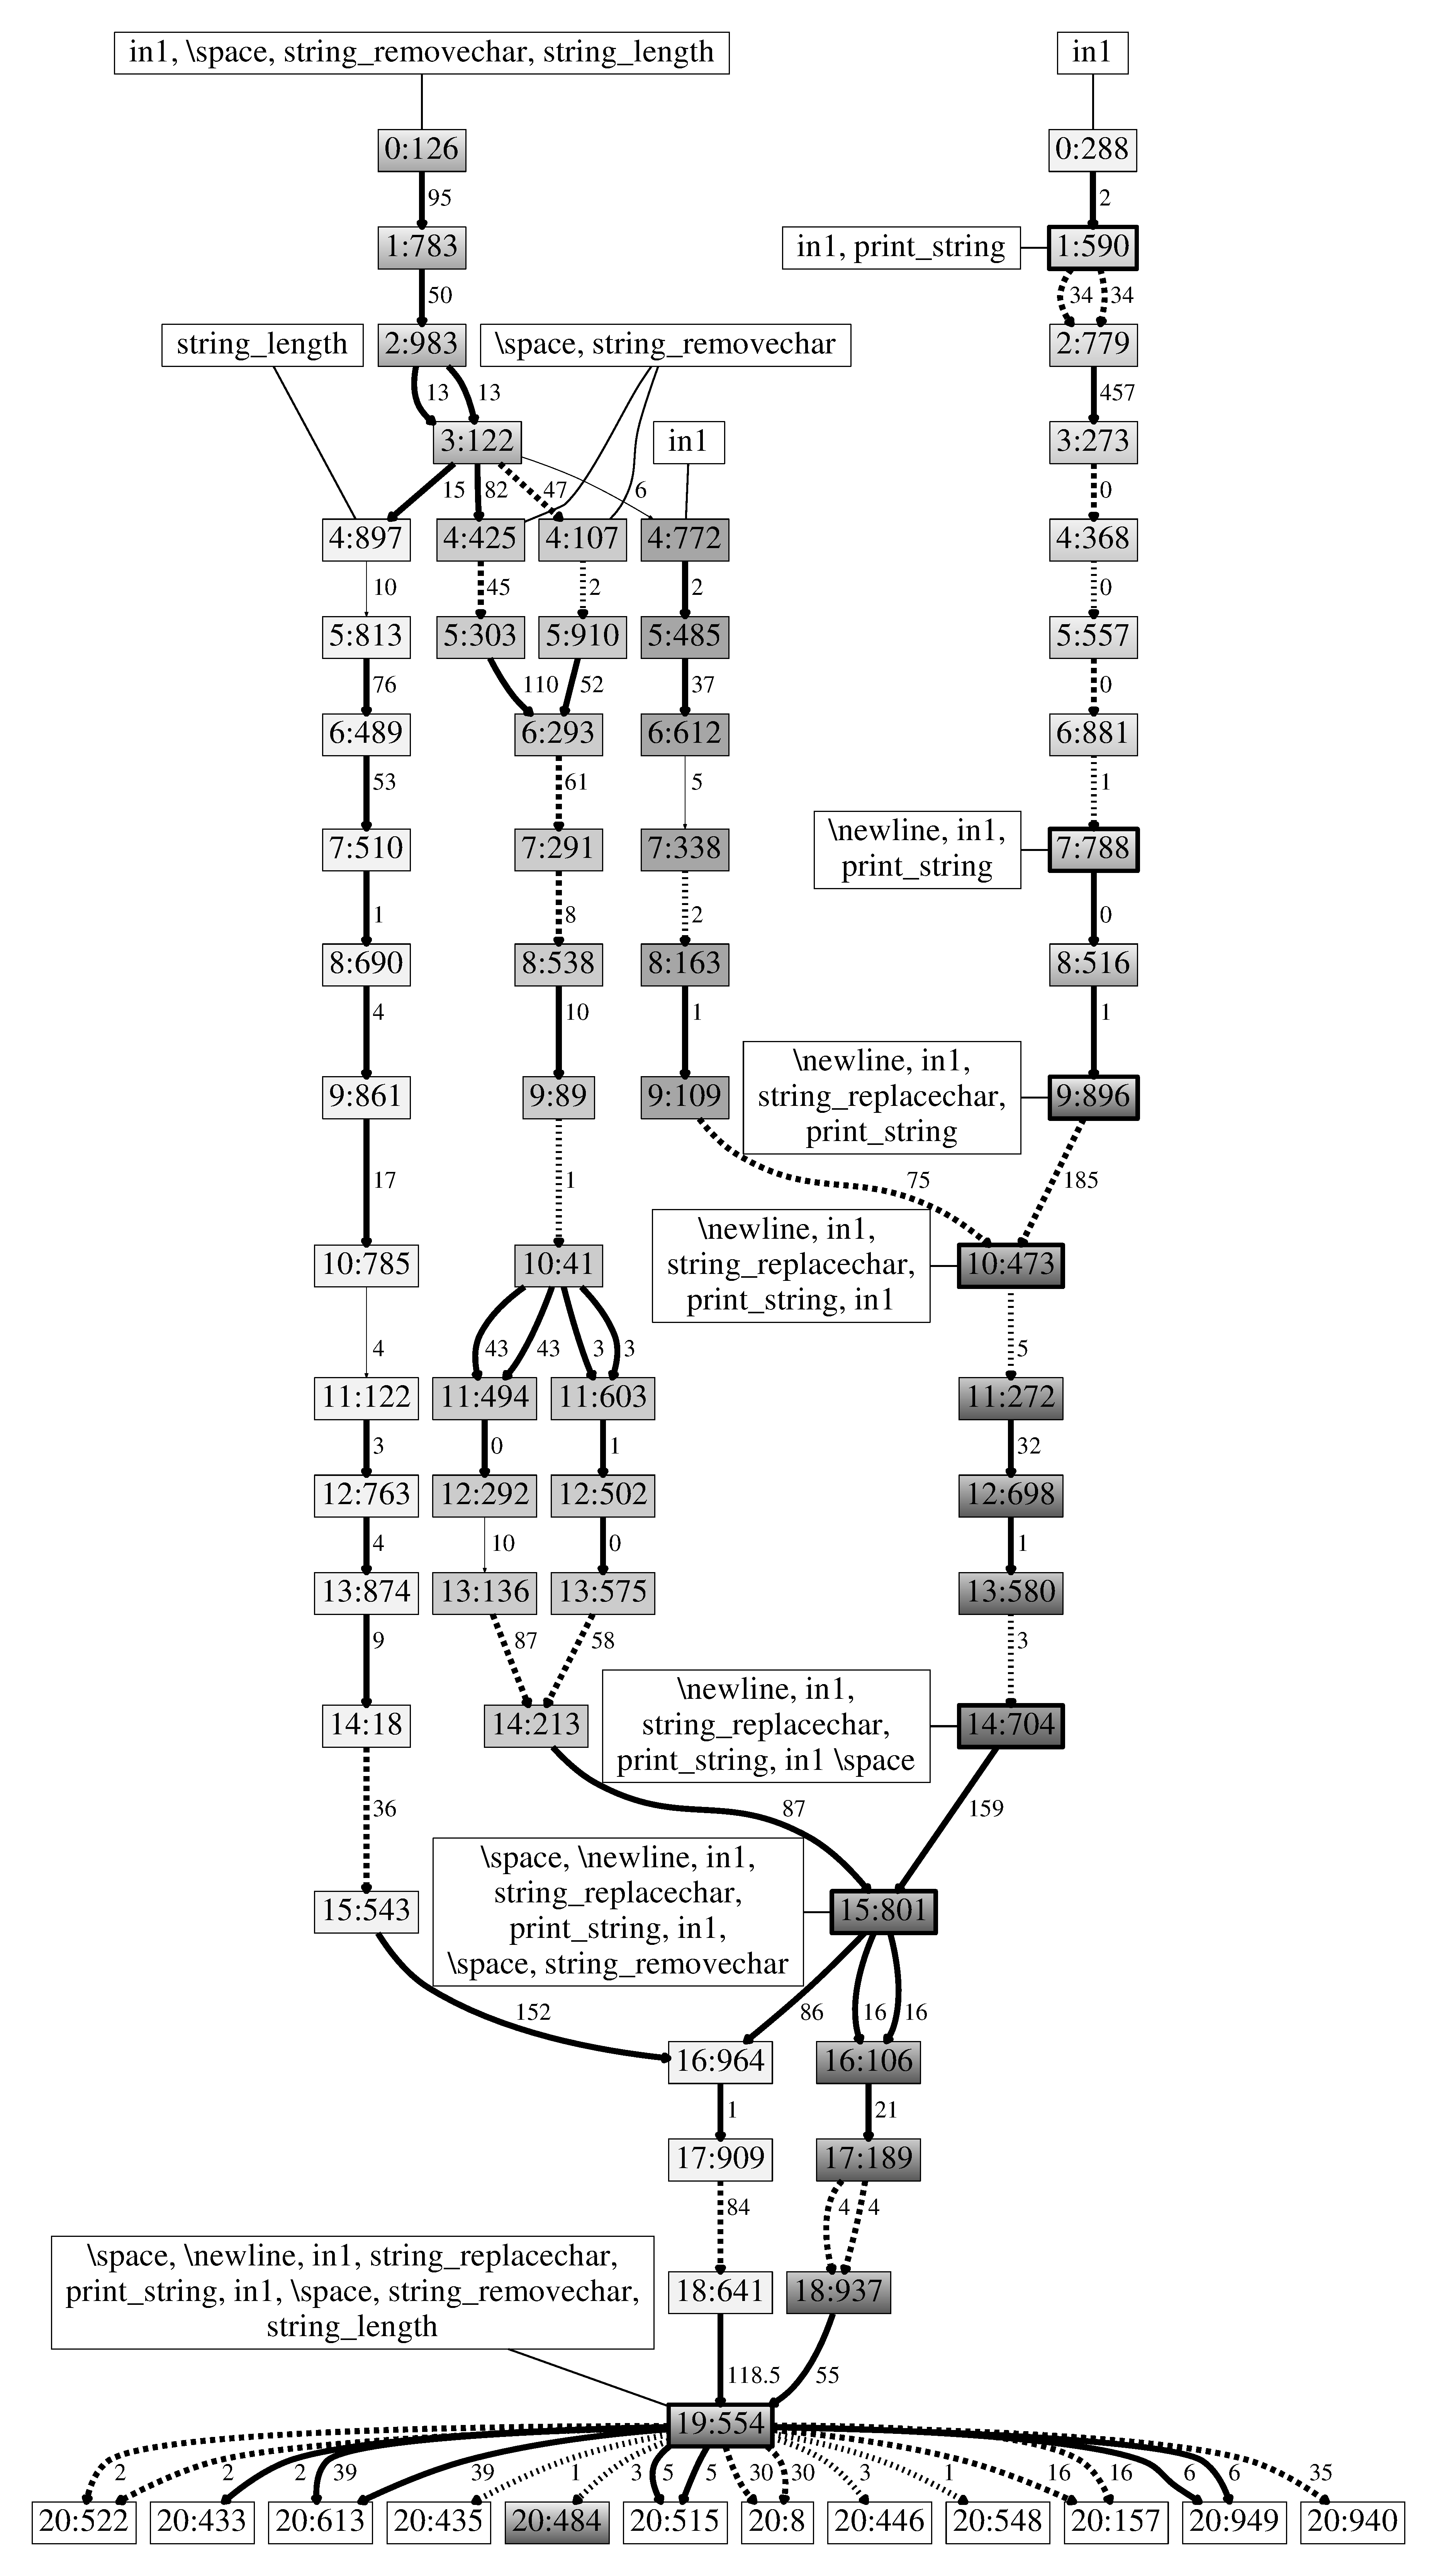
\includegraphics[height = 0.8 \textheight]{../../figures/filtered_fill.pdf}
		\end{column}
		
		\begin{column}{0.6 \linewidth}
			All 4 ``returning''instructions were present in the initial generation in right order and rough proximity in the genome
			\linespace
			Good, but lots of non-zero error; selected 45 times as a parent. 0:272 )was selected \textbf{762} times but contributed none of the key instructions to the winner (so not in graph).
			\linespace
			\textbf{Walk folks through the left hand branch(es) in the graph}
		\end{column}
	\end{columns}
\end{frame}

\subsection{It's mostly ``mutations''}

\begin{frame}{Plenty of alternation}
	\begin{center}
			\begin{tabular}{lrrr}
				\textbf{Genetic operator} & \textbf{Entire run} & \; \textbf{Full graph} & \; \textbf{Ancestry graph} \\ 
				\hline
				Alt + mutation & 9,985 (50\%) & 186 (49\%) & 39 (54\%) \\ 
				Alternation & 4,001 (20\%) & 67 (18\%) & 17 (24\%) \\ 
				Mutation & 4,026 (20\%) & 83 (22\%) & 11 (15\%) \\ 
				Close mutation & 1,988 (10\%) & 40 (11\%) & 5 (7\%)
			\end{tabular} 
	\end{center}
\end{frame}

\begin{frame}{But DL-distances tended to be small}
	
	Parent-child Damerau-Levenshtein distances in the filtered ancestry graph are typically \emph{quite} small.
	
	\vspace{-0.25 cm}
	
	\begin{center}
%	\begin{tabular}{lrrr}
%		\textbf{Genetic operator} & \textbf{Entire run} & \; \textbf{Full graph} & \; \textbf{Ancestry graph} \\ 
%		\hline
%		Alt + mutation & 9,985 (50\%) & 186 (49\%) & 39 (54\%) \\ 
%		Alternation & 4,001 (20\%) & 67 (18\%) & 17 (24\%) \\ 
%		Mutation & 4,026 (20\%) & 83 (22\%) & 11 (15\%) \\ 
%		Close mutation & 1,988 (10\%) & 40 (11\%) & 5 (7\%)
%	\end{tabular} 
		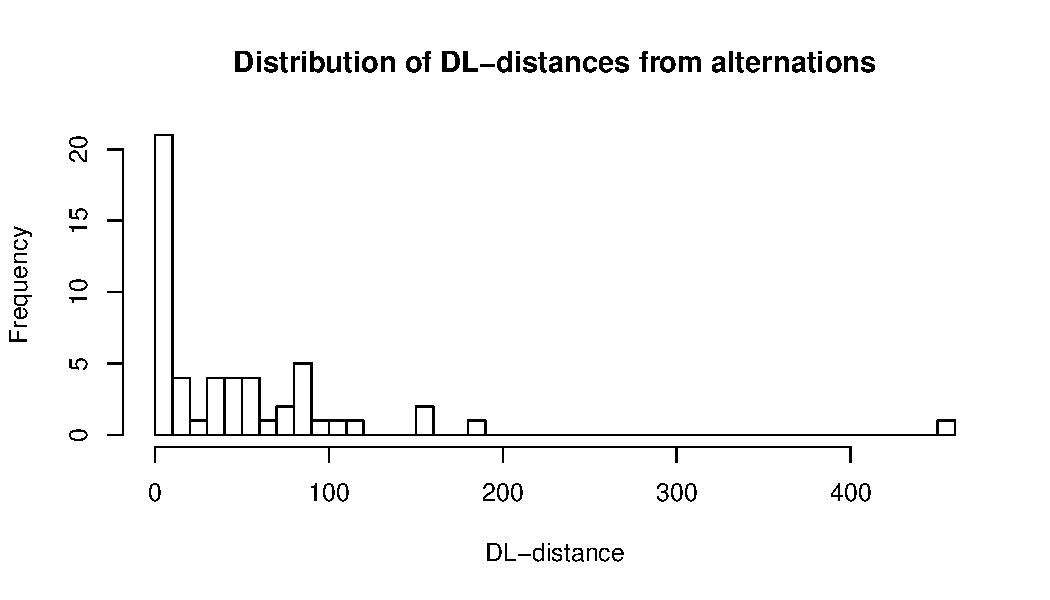
\includegraphics[width=\textwidth]{../../figures/Alternation_dl_distance_distribution}
	\end{center}
\end{frame}

\begin{frame}{But some ``real'' crossovers}
	\textbf{Walk through alternation that created 15:801}
\end{frame}

\section[Conclusions]{Conclusions}

\begin{frame}
\frametitle{Conclusions}

\begin{itemize}
\item We did it!
\item Time consuming/labor intensive, though
\item Found interesting beetles, e.g.,
\begin{itemize}
	\item Role of mutation
	\item Low DL-distances
\end{itemize}
\end{itemize}

\linespace
\linespace

Future Work
\begin{itemize}
\item Automate more of the work
\item Take a run and generate a simple report fully automatically
\item Add UUIDs to genes to simplify tracking and make it more accurate
\end{itemize}
\end{frame}

\begin{frame}{Thanks!}
	
	Thank you for your time and attention!

	\linespace
	
	Thanks to Lee Spector's Computational Intelligence group (Hampshire College) and Bill Tozier for ideas and feedback, and Bill Tozier, Stephan Winkler, and Wolfgang Banzhaf for their feedback on the submitted draft of this paper.
		
	\linespace
	\linespace
	
	\begin{center}
	{\huge Questions?}
	\end{center}
\end{frame}

%\section*{References}
%
%\begin{frame} 
%\frametitle{References}
%\bibliographystyle{apalike}
%{\tiny \bibliography{GraphDBandGP}}
%\end{frame} 

\end{document}


